\section{Can I Rely On You - appendix}\label{appendix:can-i-rely}

\subsection*{Attribution Examples}\label{appendix:attribution-examples}

Because the amount of attribution examples is to large to fit them in the appendix, they are available at \url{https://drive.google.com/drive/folders/177nMz2Y21Z505Eb5r8NZwAMQoMfX6S5f?usp=sharing} (total number of files equals $23150$). File structure is following the pattern \verb|{{Dataset}/{Model version}/{XAI method}|. Each image has a filename containing:

\verb|{index}-{true class}-{predicted class}.png|

\subsection{Infidelity - combined scores}\label{appendix:combined-inf}

Individual scores can be find at \url{https://drive.google.com/drive/folders/1_0PaXj2QbuW5DyAFjlrKAUjJ_iaoEn9a?usp=sharing}. Folder "\textbf{individual}" contains separated scores per dataset/model. Folder "\textbf{combined}" contains combined scores. Folder "\textbf{confidence}" contains infidelity values with standard deviation values.

\begin{figure}[ht]
  \centering
  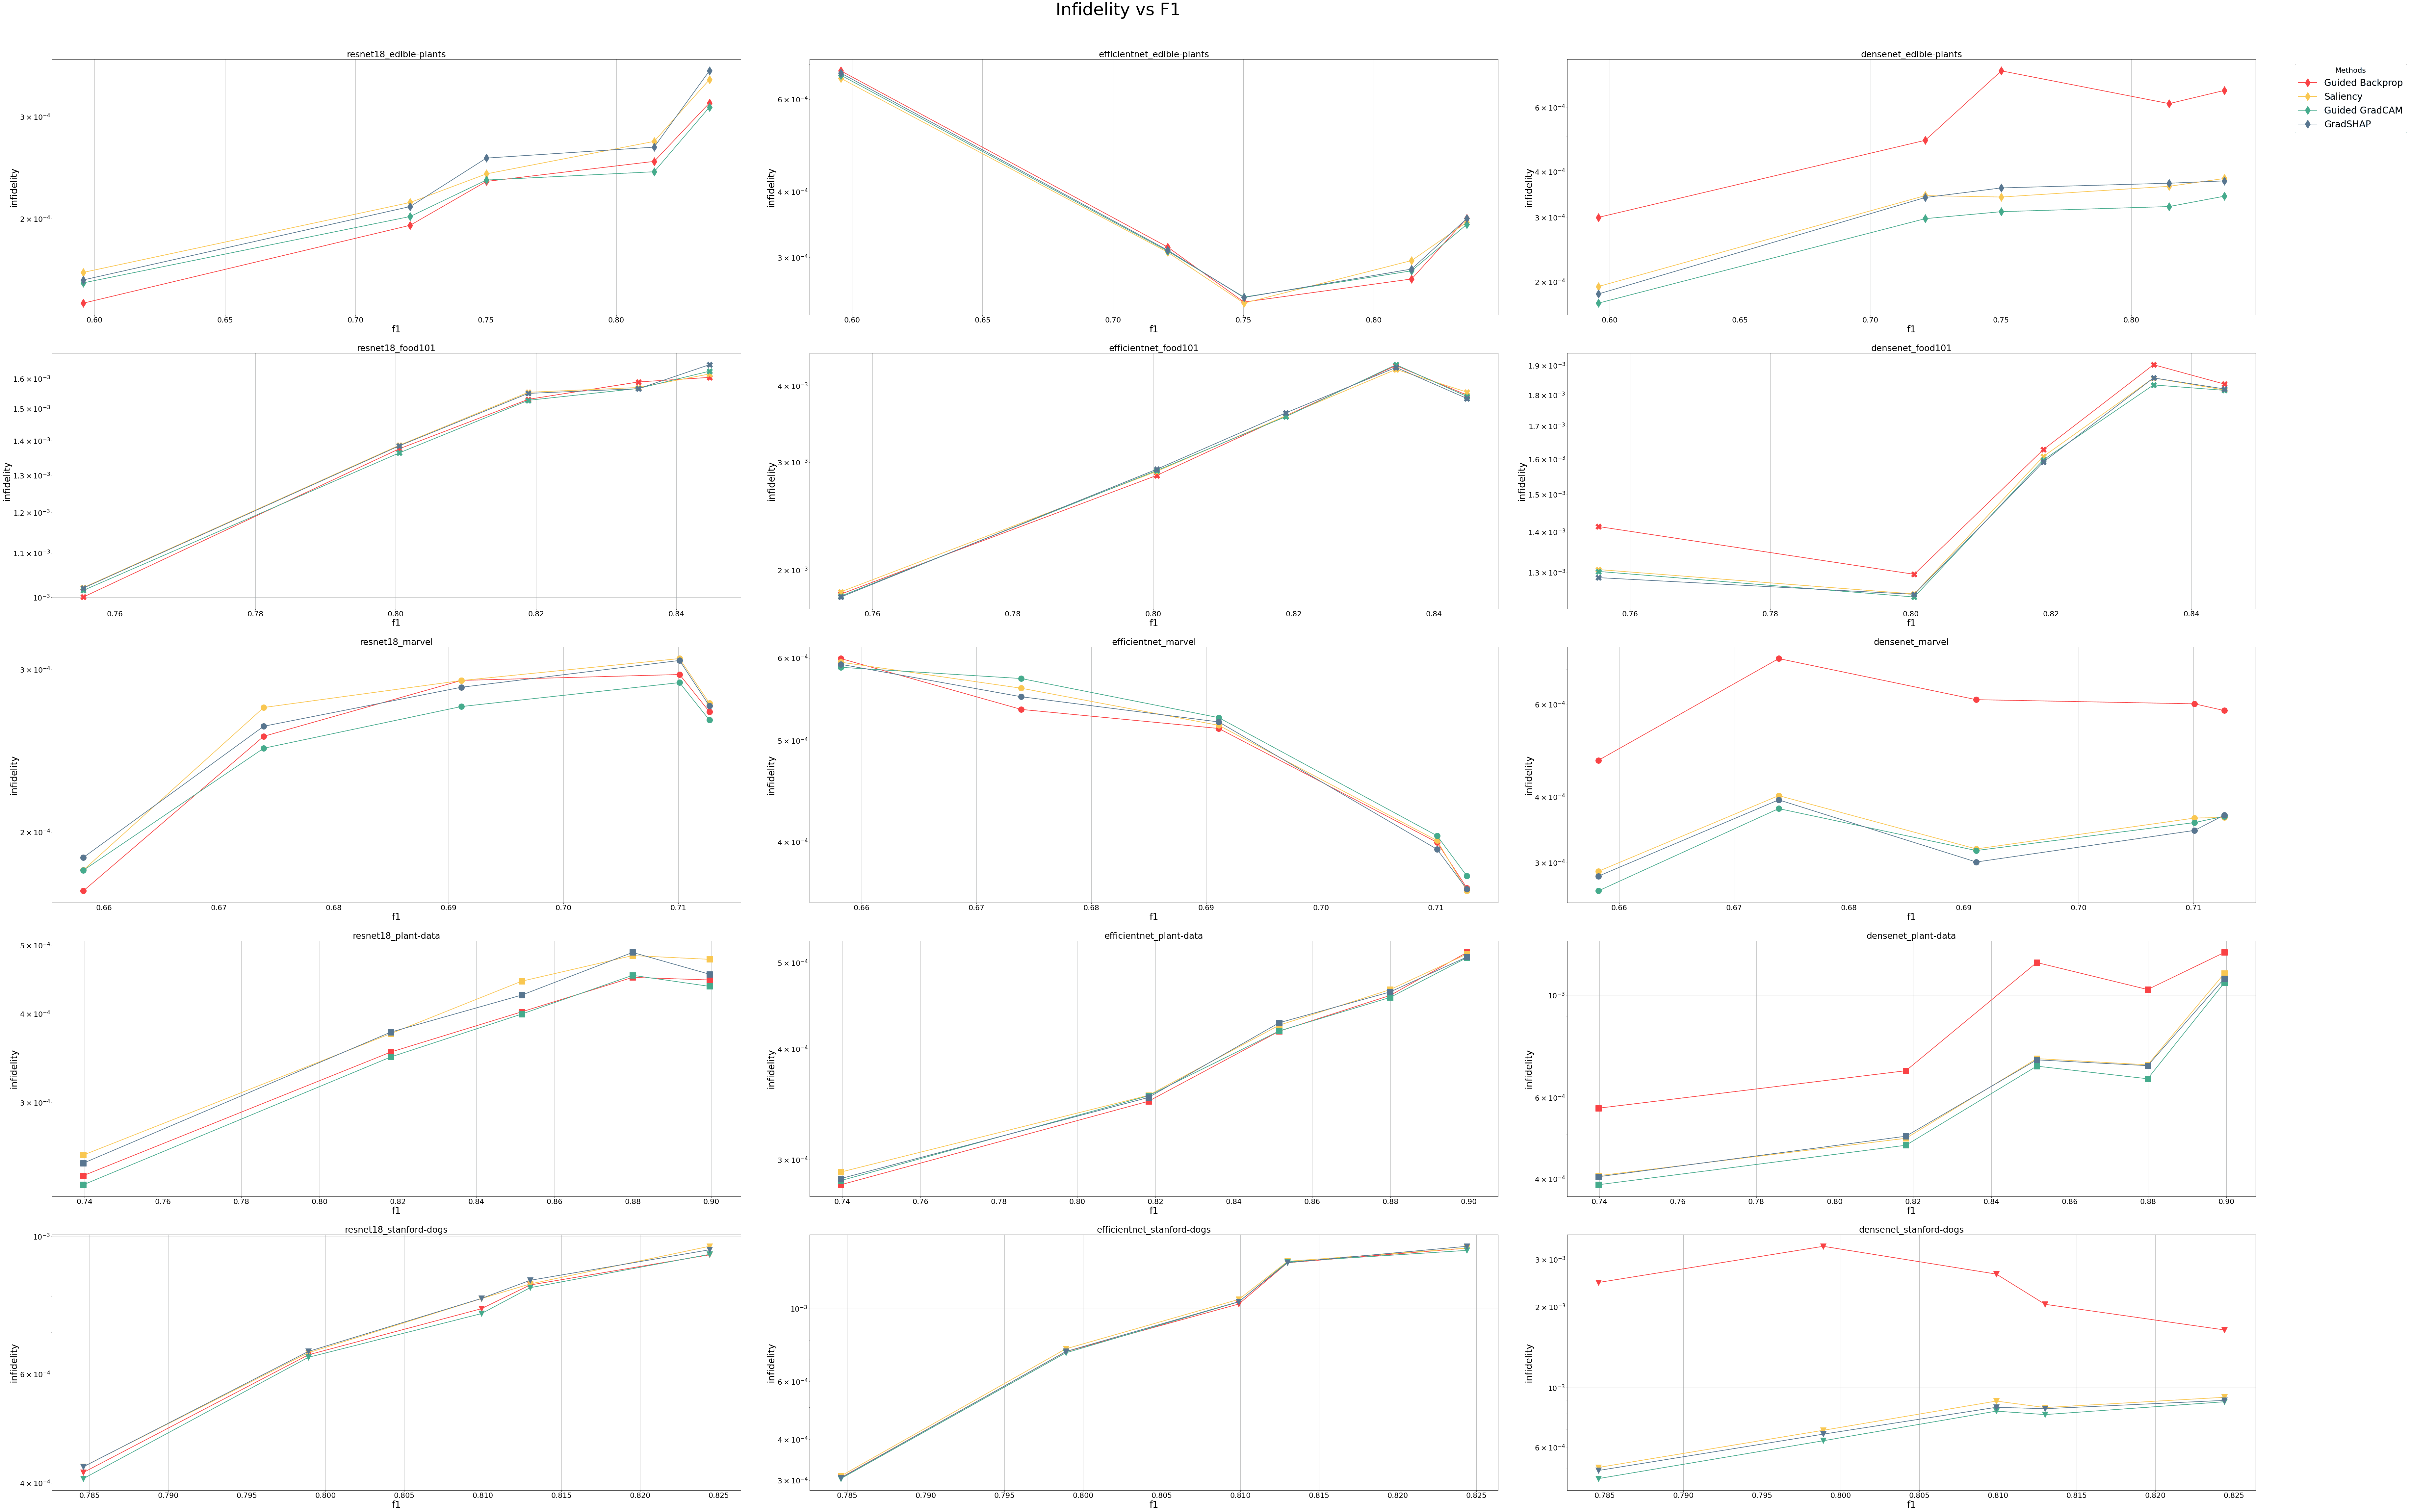
\includegraphics[width=\textwidth]{appendixes/images/inf-combined-f1.png}
  \caption{Combined Infidelity scores against F1 scores. Each row represents a dataset, each column represents an architecture (see individual subplot titles)}\label{fig:combined-infidelity}
\end{figure}

\begin{figure}[ht]
  \centering
    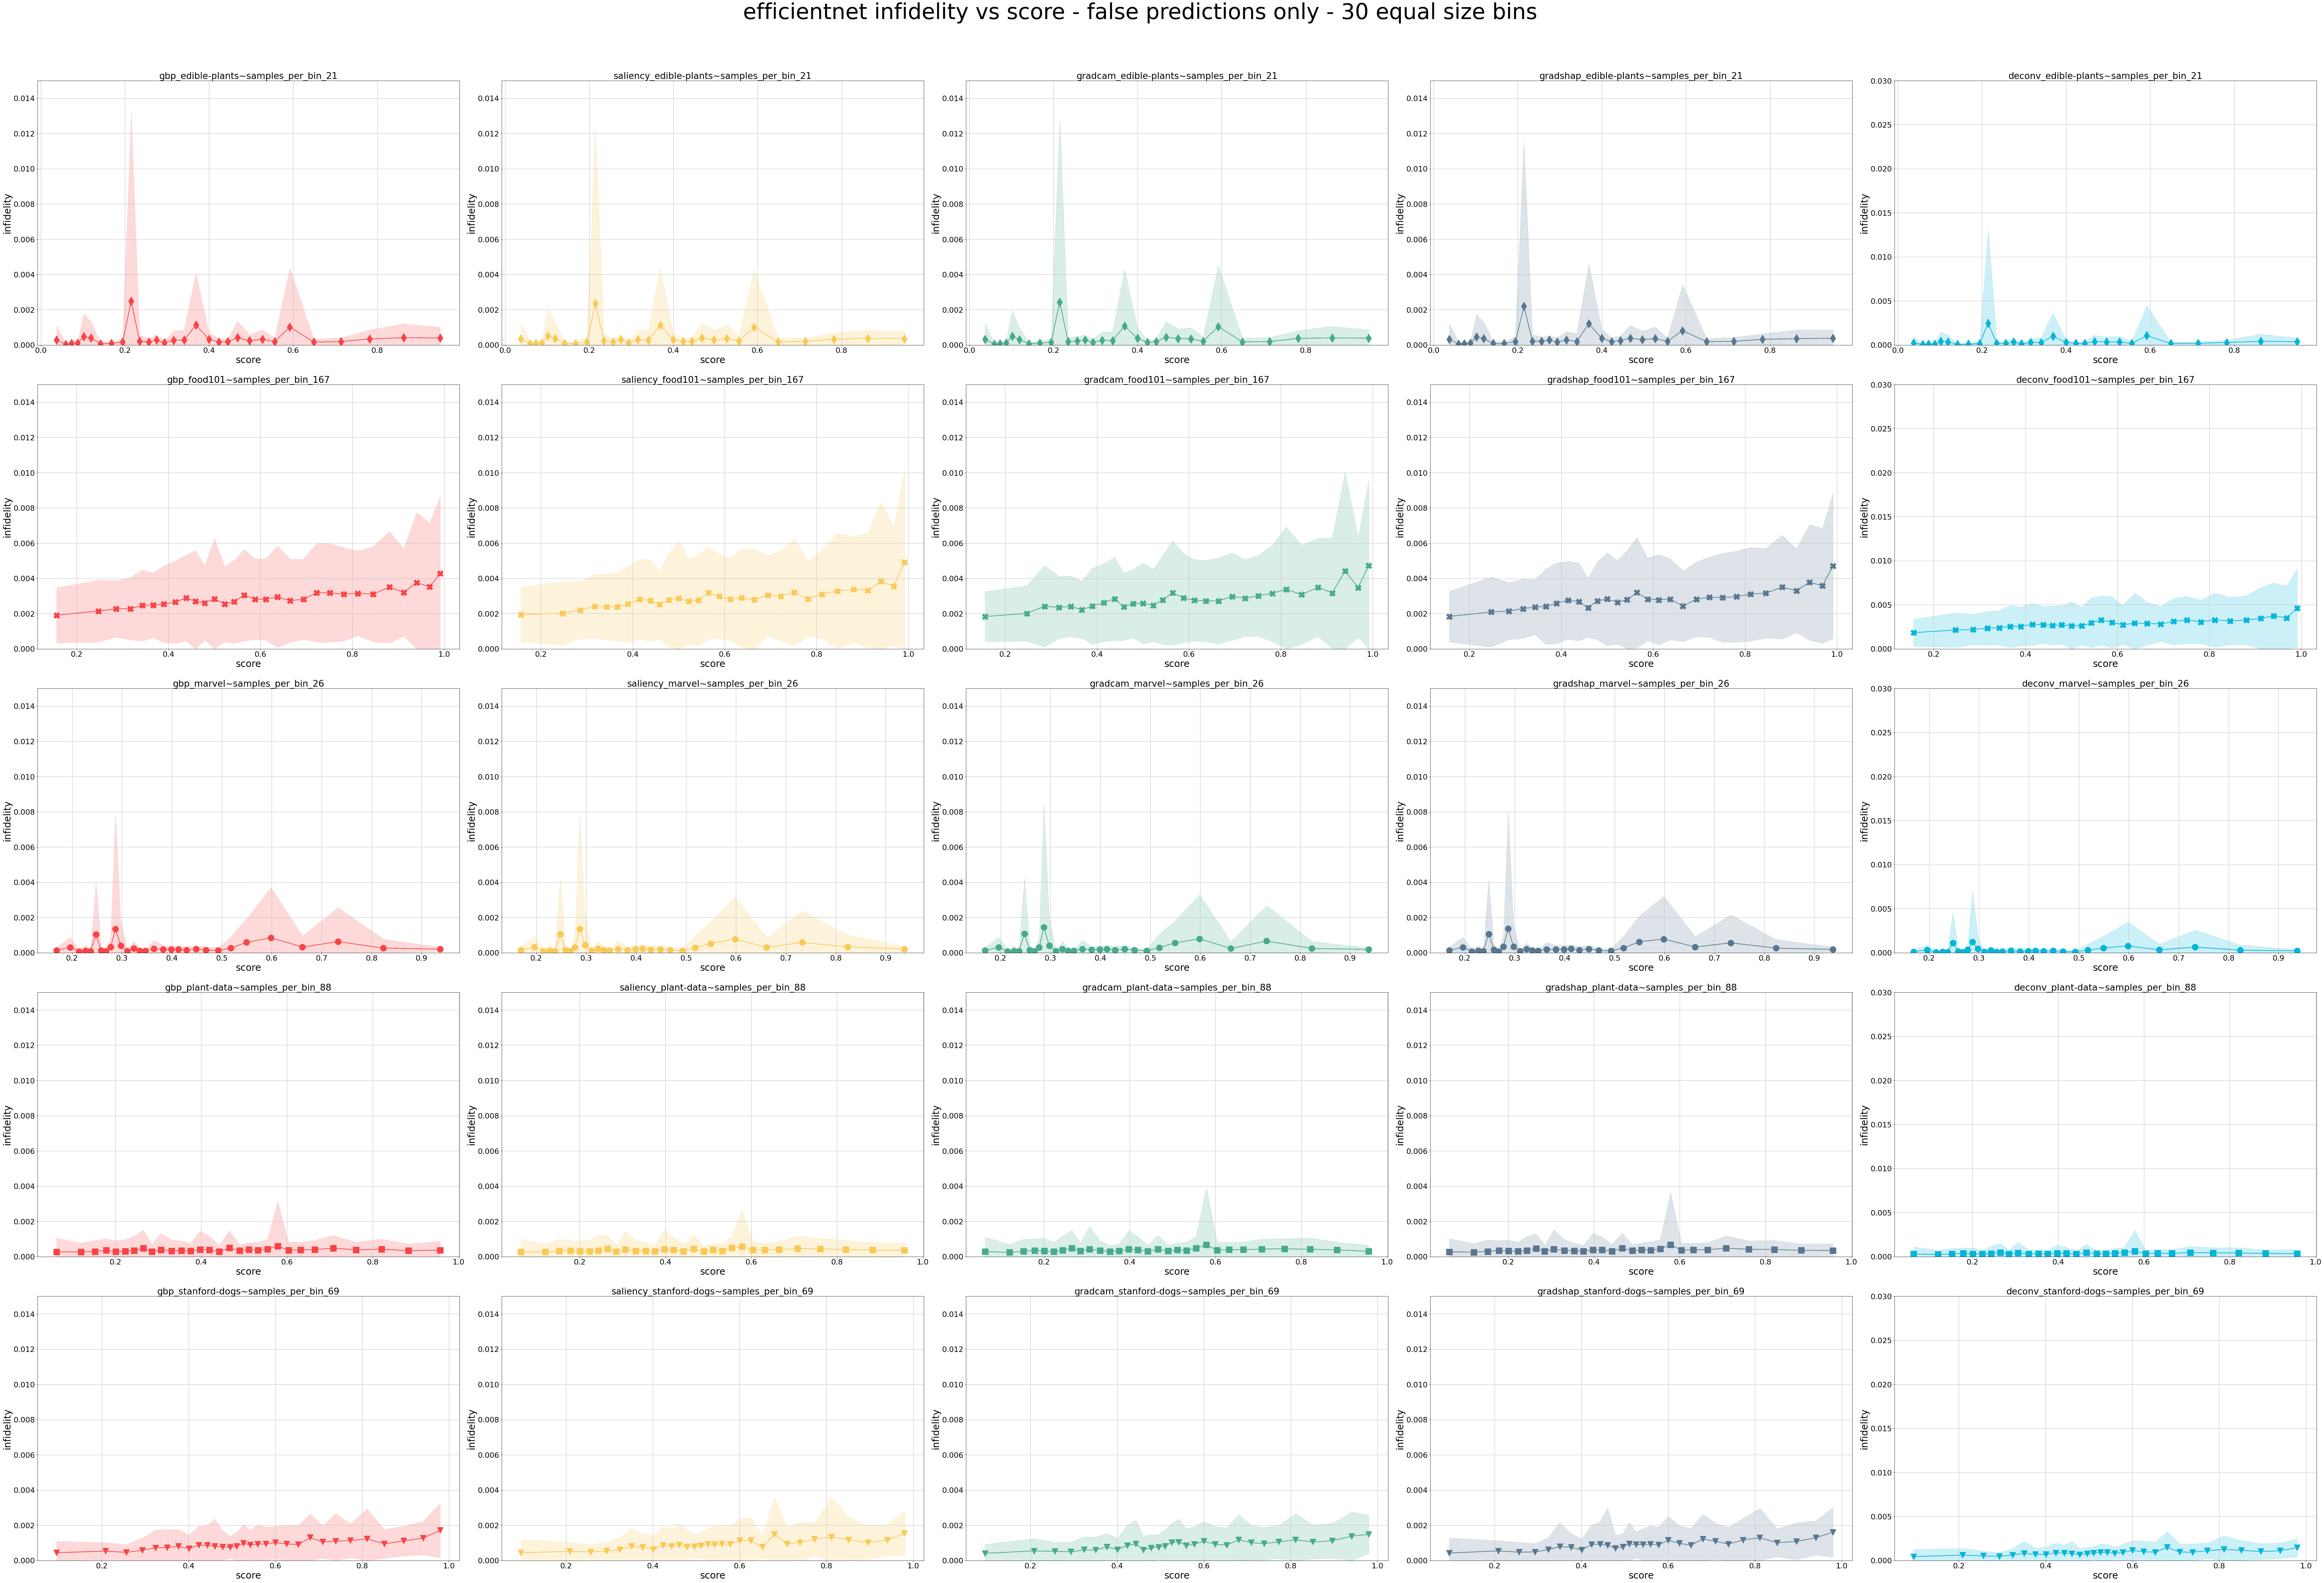
\includegraphics[width=\textwidth]{appendixes/images/efficientnet-infidelity vs score - false predictions only - 30 equal size bins.png}
    \caption{Infidelity scores (with standard deviation) on \textit{EfficientNet B0} architecture. All scores are the mean value for the particular model and are related to that models' predicted scores (x-axis). Each data point is a mean value of the same amount of samples per dataset. Amounts differ between datasets to always split the results into 30 equally-sized bins.}\label{fig:efficientnet-inf-std}
\end{figure}


\begin{figure}[ht]
  \centering
    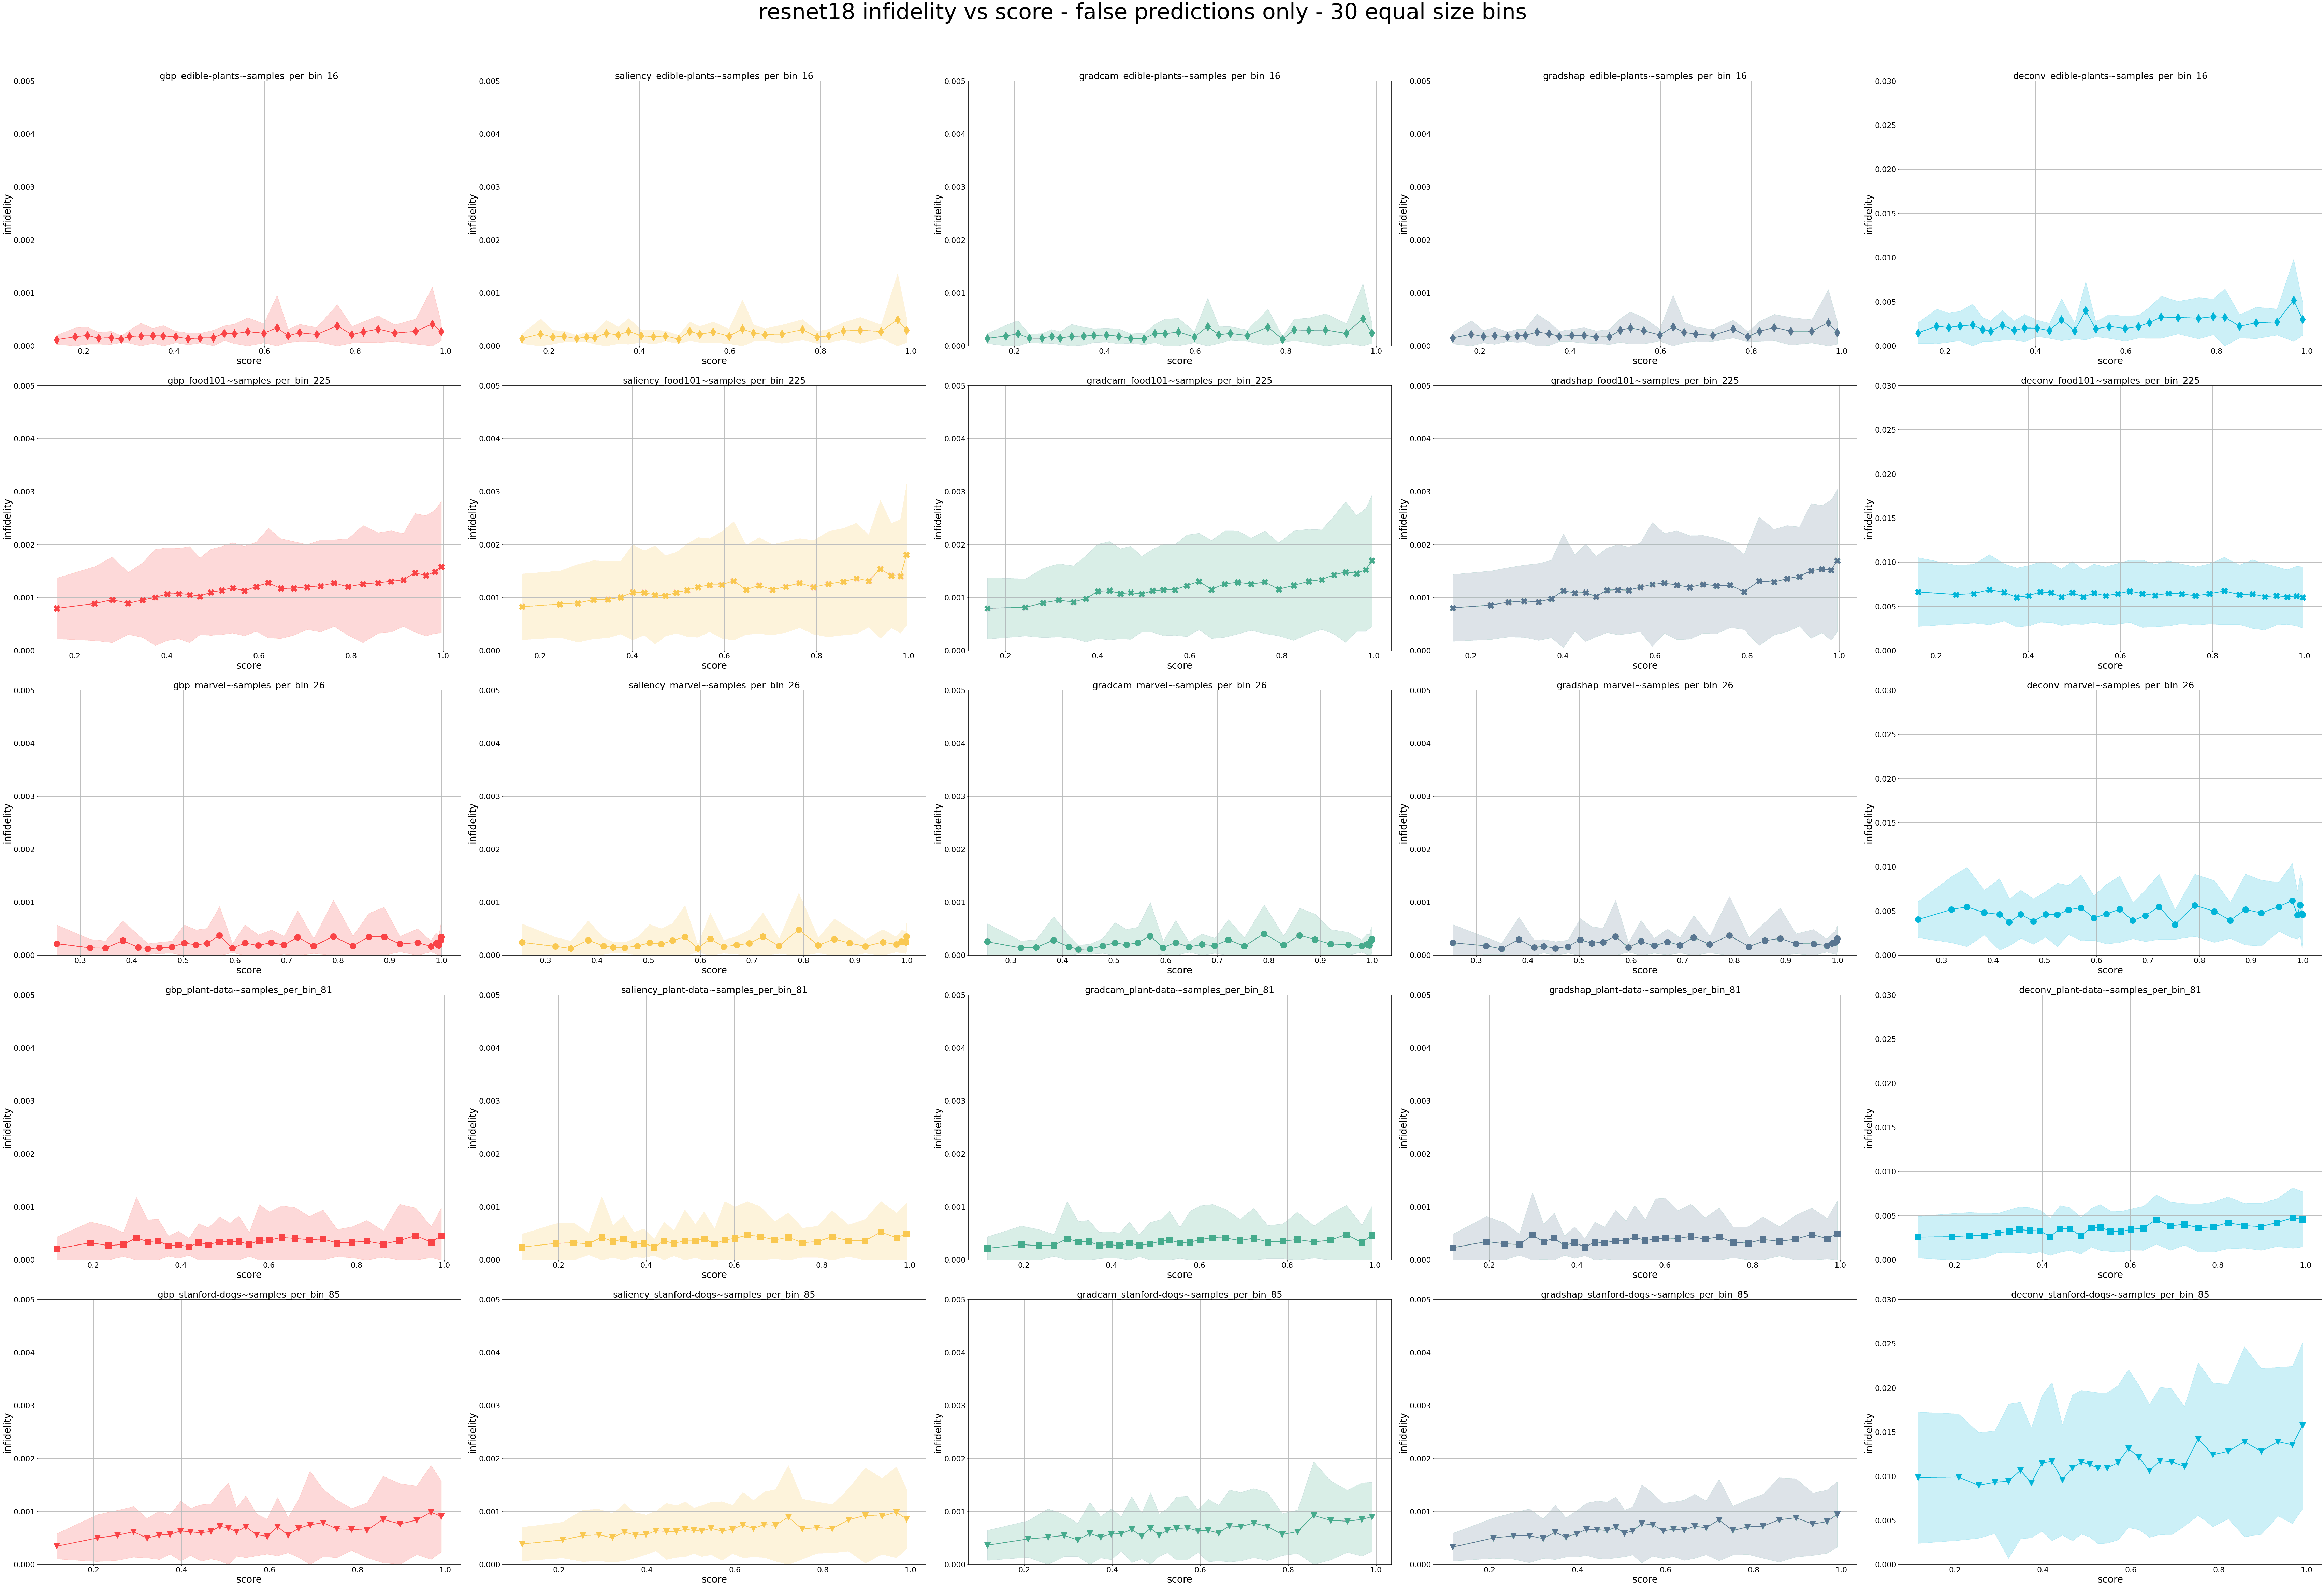
\includegraphics[width=\textwidth]{appendixes/images/resnet18-infidelity vs score - false predictions only - 30 equal size bins.png}
    \caption{Infidelity scores (with standard deviation) on \textit{ResNet18} architecture. All scores are the mean value for the particular model and related to that models' predicted scores (x-axis). Each data point is a meas value of the same amount of samples per dataset. Amounts differ between datasets to always split the results into 30 equally-sized bins.}\label{fig:resnet-inf-std}
\end{figure}

\subsection{Sensitivity - combined scores}\label{appendix:combined-sens}

Individual scores can be find at \url{https://drive.google.com/drive/folders/12eYJSZFMfI2FZhXQSuwJQ6I8w65EU25e?usp=sharing}. Folder "\textbf{individual}" contains separated scores per dataset/model. Folder "\textbf{combined}" contains combined scores. Folder "\textbf{confidence}" contains sensitivity values with standard deviation values.

\begin{figure}[ht]
  \centering
  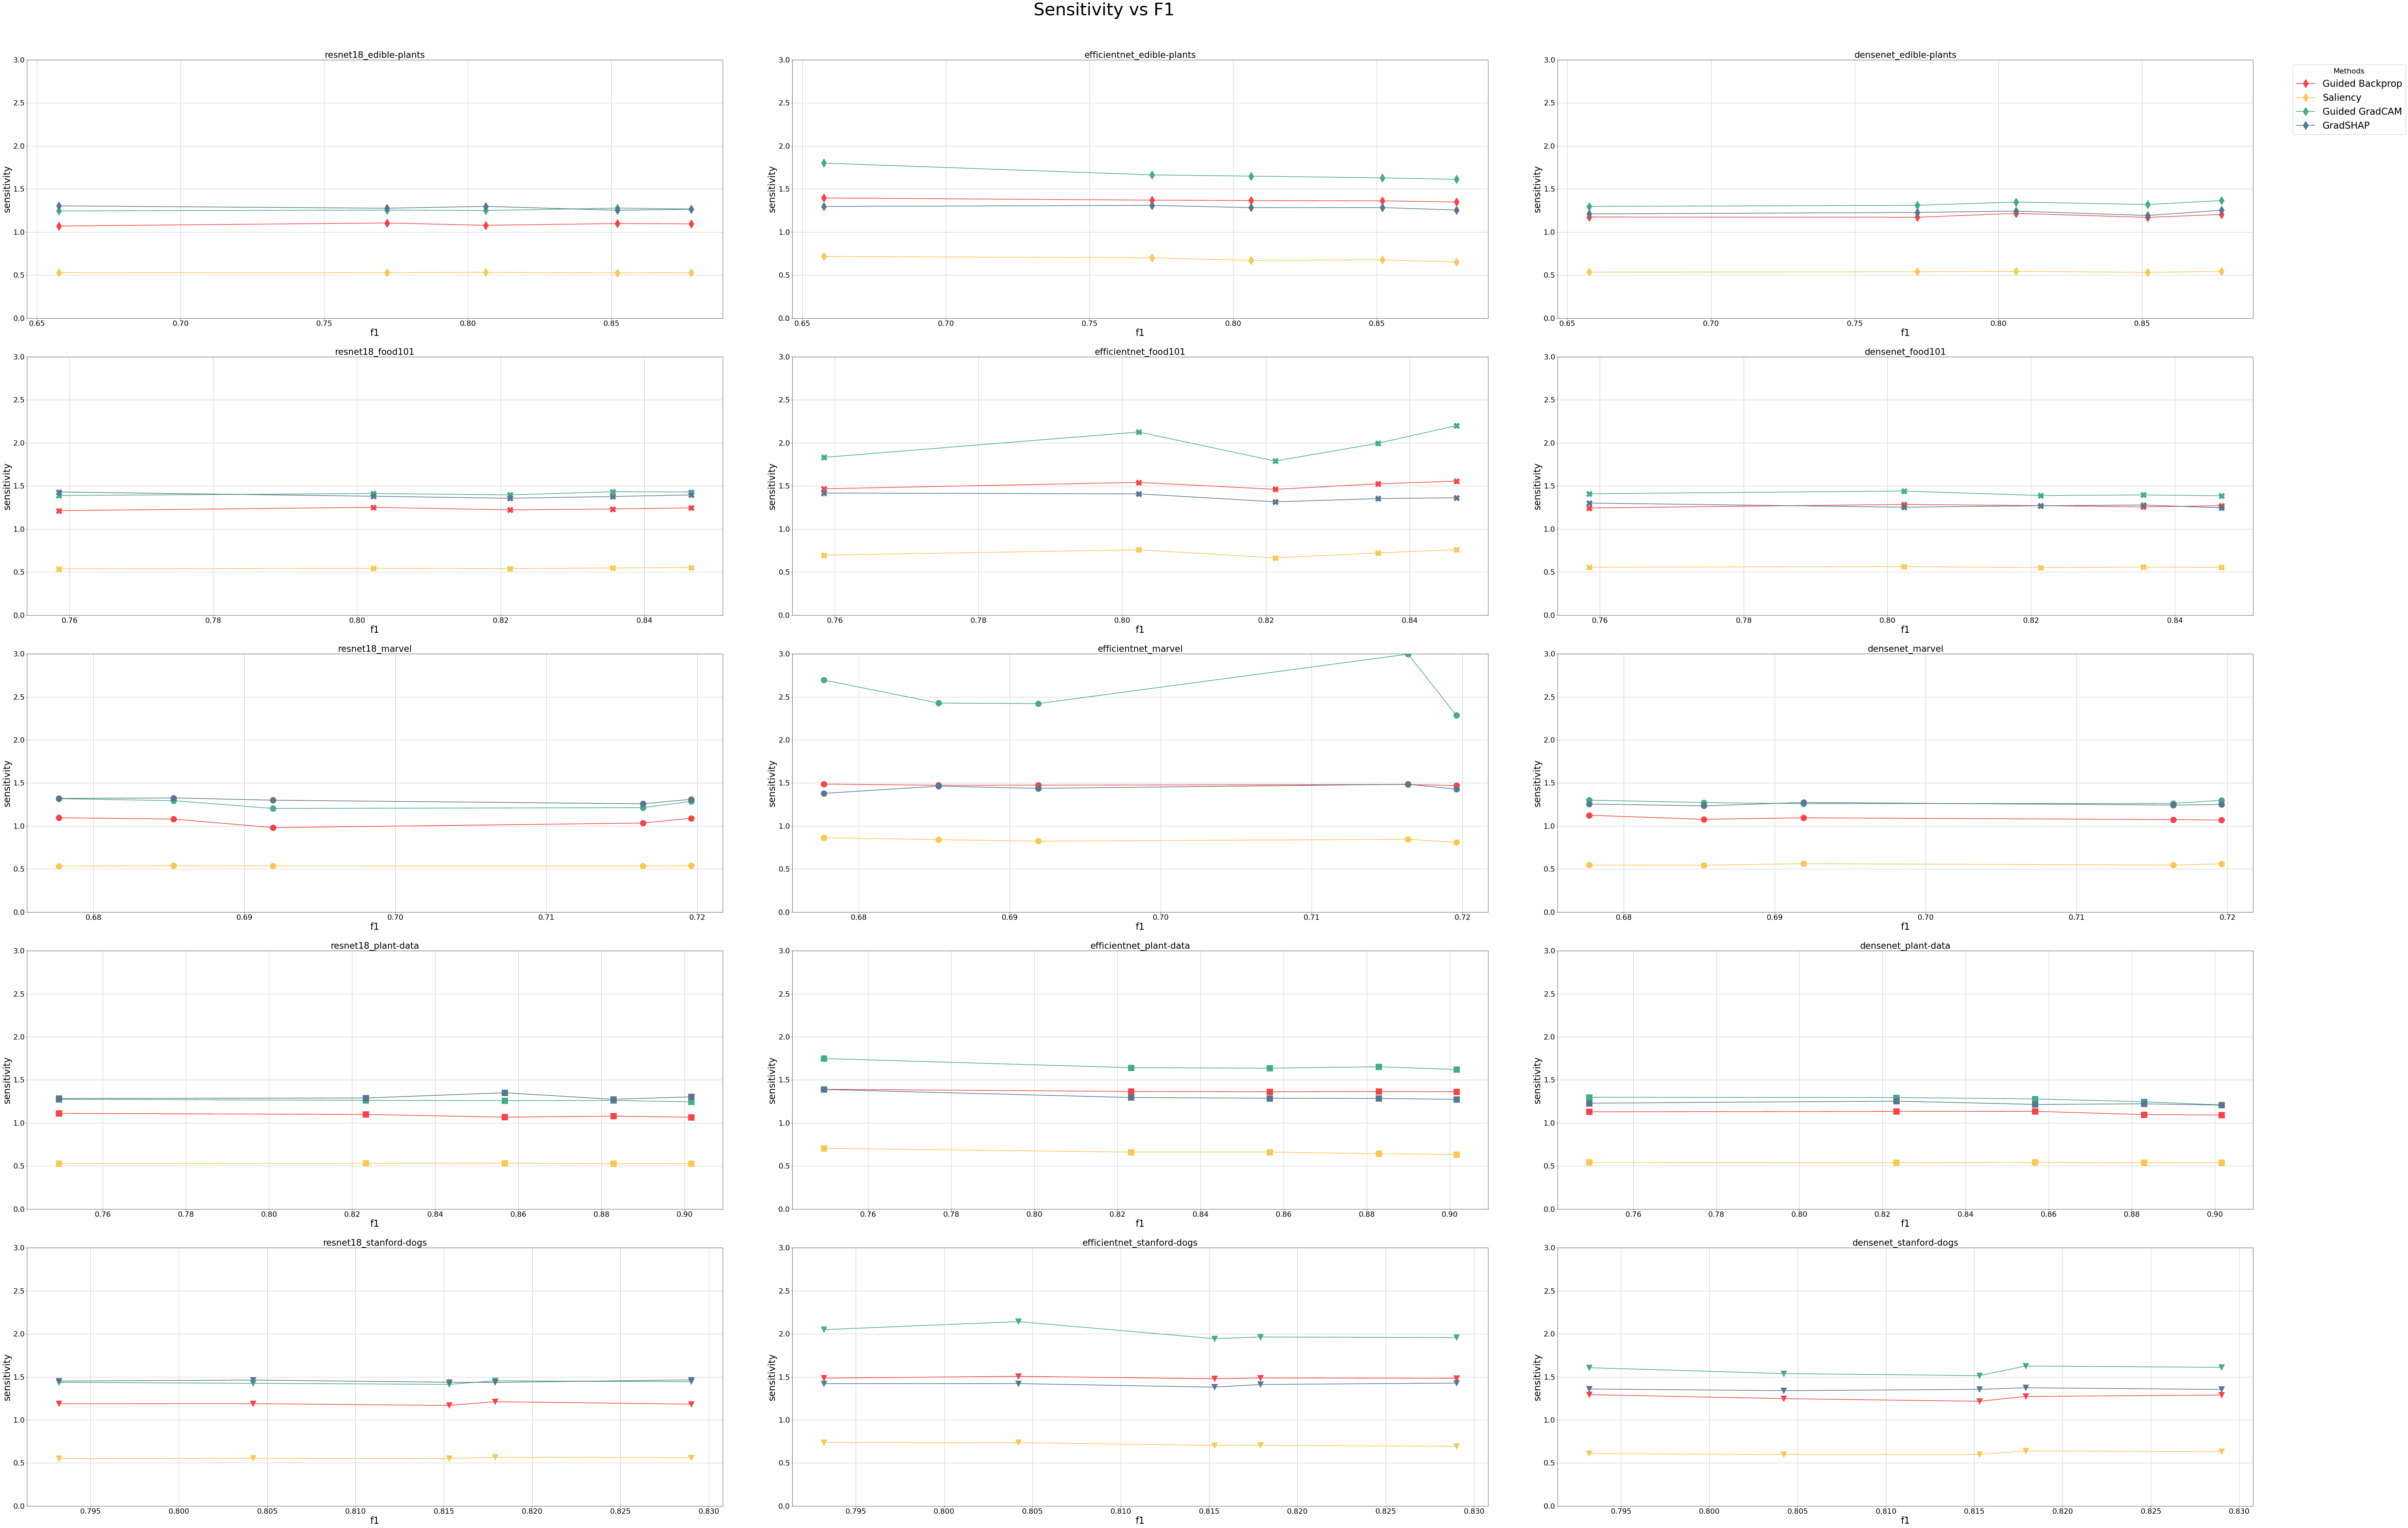
\includegraphics[width=\textwidth]{appendixes/images/sensitivity-combined-f1.png}
  \caption{Combined Sensitivity scores against F1 scores. Each row represents a dataset, each column represents an architecture (see individual subplot titles)}\label{fig:combined-sensitivity}
\end{figure}

\begin{figure}[ht]
  \centering
    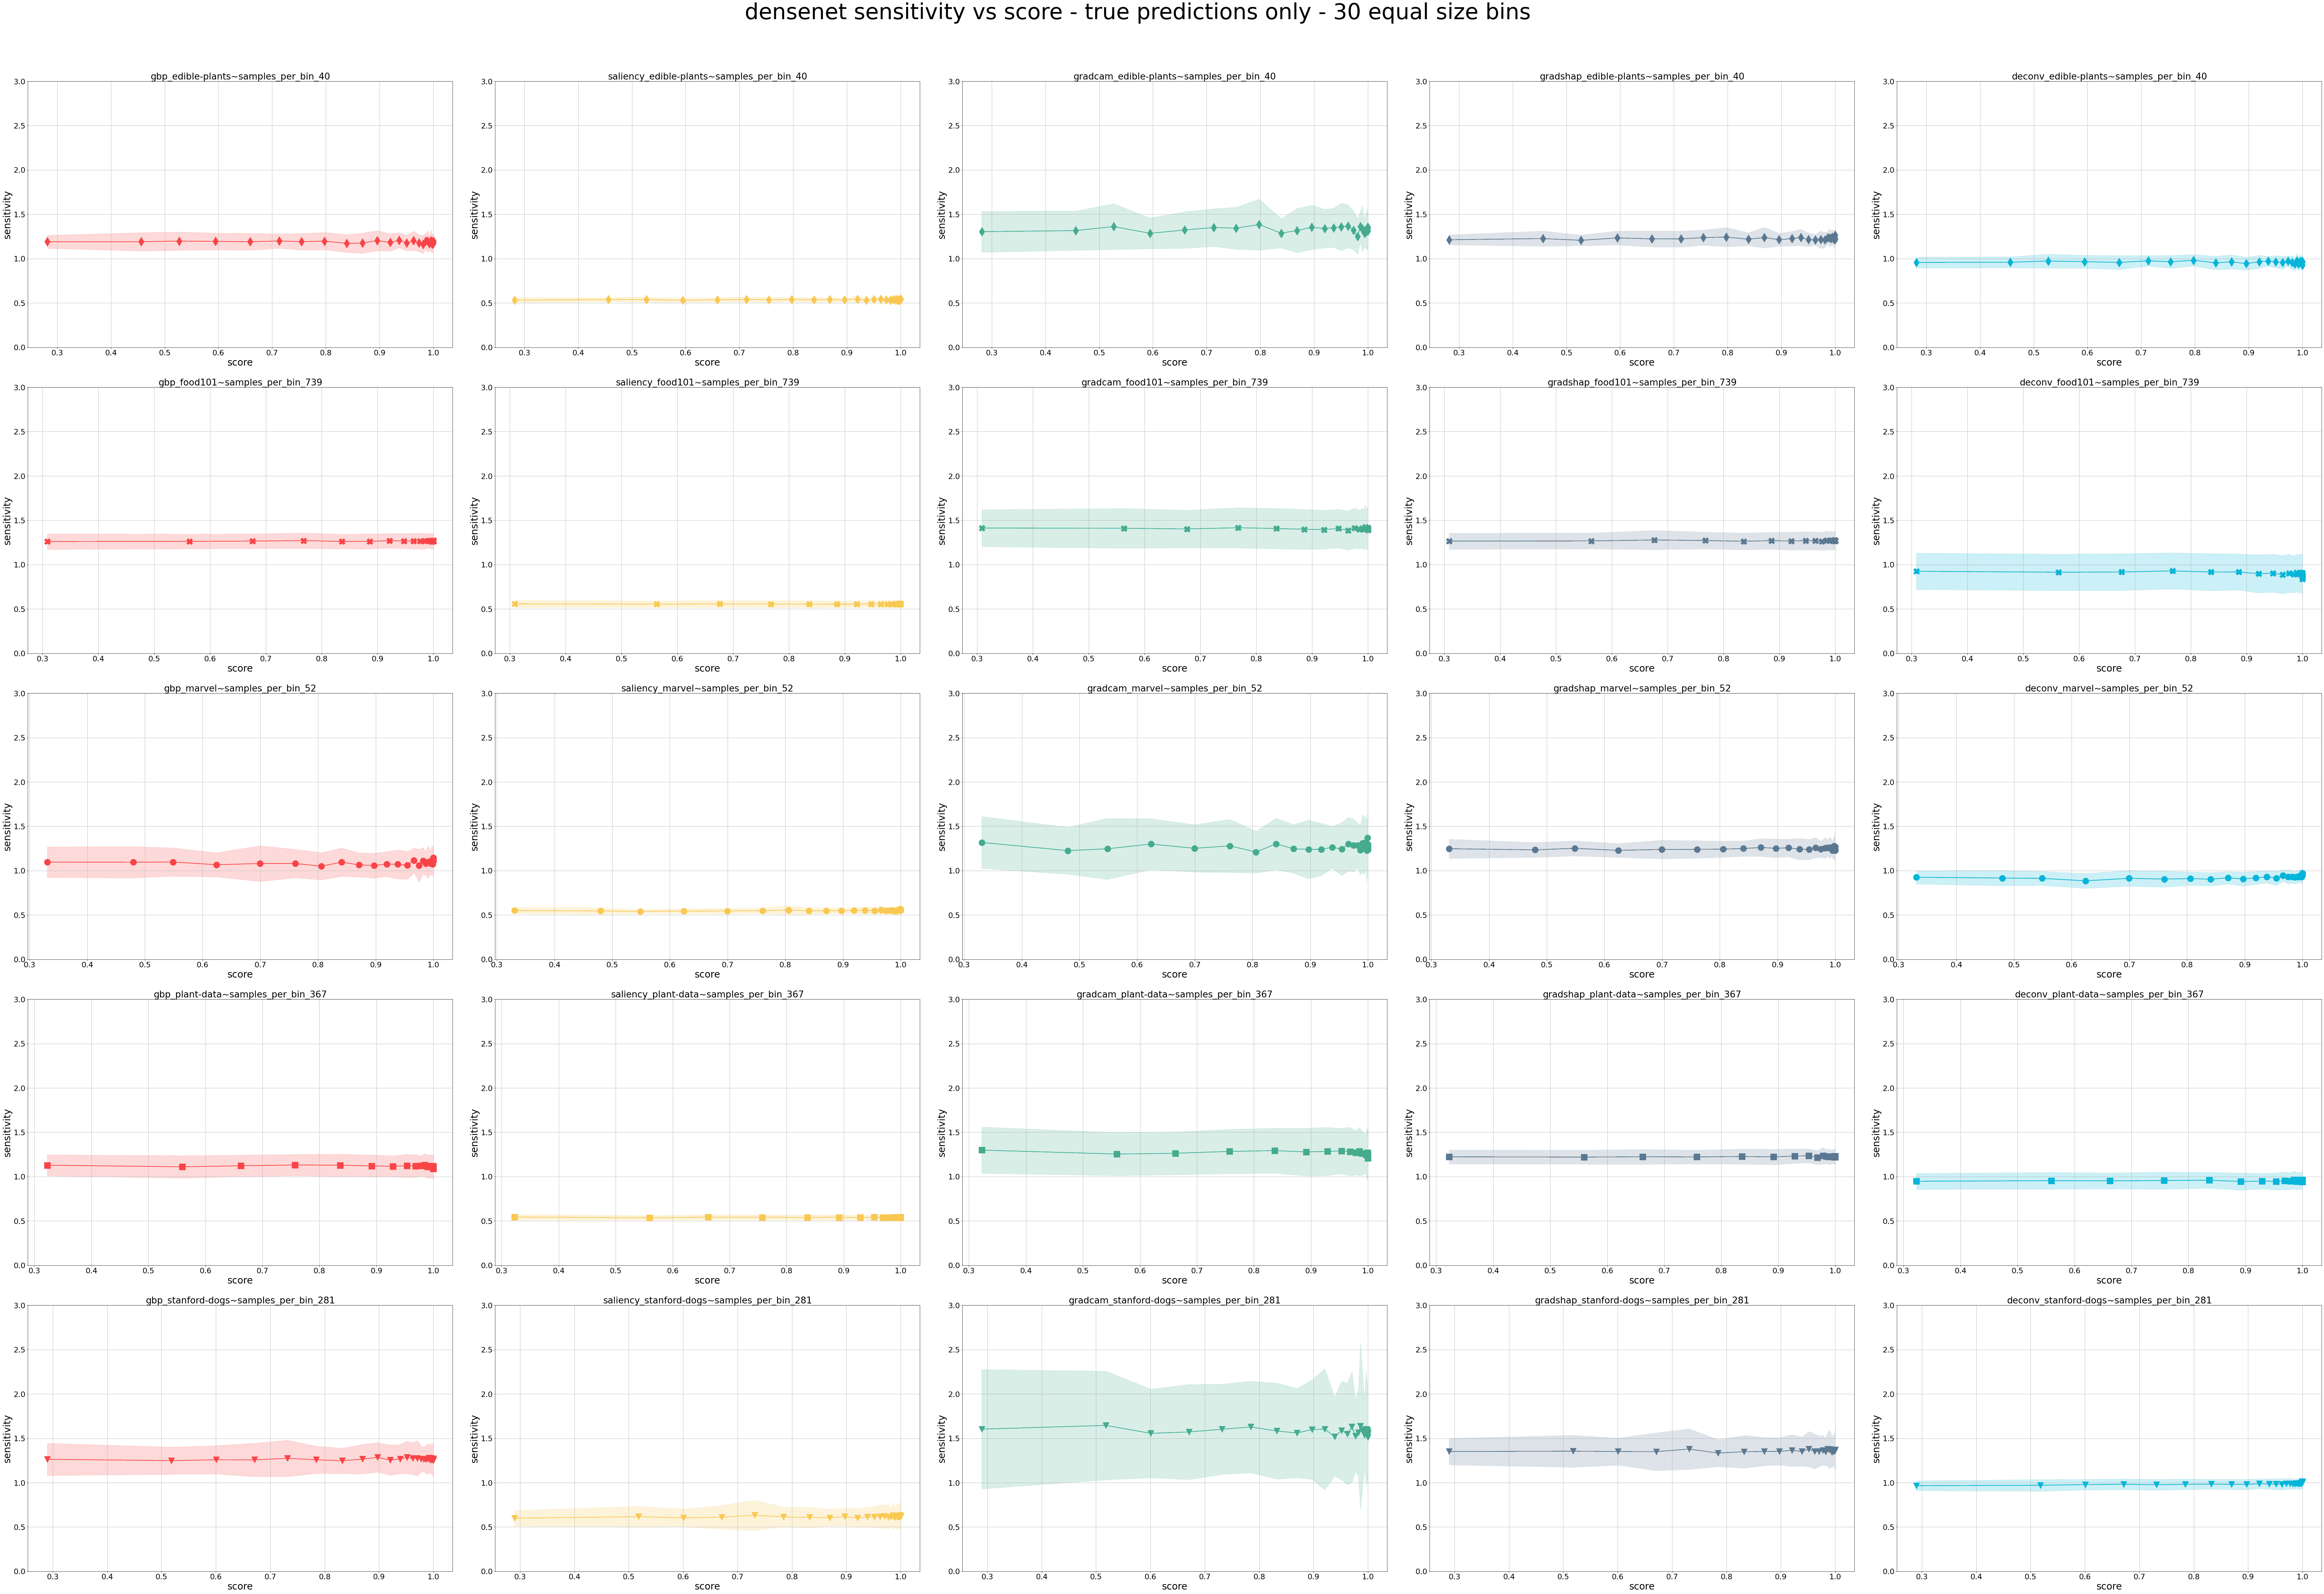
\includegraphics[width=\textwidth]{appendixes/images/densenet-sensitivity vs score - true predictions only - 30 equal size bins.png}
    \caption{Sensitivity scores (with standard deviation) on \textit{DenseNet121} architecture. All scores are the mean value for the particular model and are related to that models' predicted scores (x-axis). Each data point is a mean value of the same amount of samples per dataset. Amounts differ between datasets to always split the results into 30 equally-sized bins.}\label{fig:densenet-sens-std}
\end{figure}